\documentclass{article}
\usepackage[utf8]{inputenc}
\usepackage{graphicx}

\title{Cloud Atlas \\[1ex] \large An LstmEncoder for UHECR AirShowers}
\author{Gianluca Becuzzi, Lucia Papalini}
\date{July 2022}

\begin{document}

\maketitle

In this project we propose an example of using deep learning techniques to predict features of UHECR 
(Ultra High Energy Cosmic Rays) Showers.
In particular when this kind of cosmic ray enters the atmosphere they produce a particle cascade 
that can be identified with a set of water-Cherenkov or scintillator ground-based detectors, and our aim
 is to train a neural network to predict the height at which the shower formed by feeding it with data 
 of the triggers of such detectors.\\
The dataset on which we perform the training consists in a simulation of an Auger-like apparatus, 
made of a 9x9 array of detectors.  Data are organised organised as follow:
%DESCRIVERE QUEI DATI DI MERDA
\\
The first step to take is the splitting of the dataset into the different features:
 the whole project is based on a custom numpy \textit{dtype} for the storage the different event's attributes
  in a single (?) sorted by \textit{toa}, \textit{time\_series} and \textit{outcome}.\\
A first sight of the dataset showed the need for augmentation of data at high values of height,
 so we built the \textit{Augmentation} class to perform that: it consists in increasing the 
 number of those data applying rotations and symmetry-flips on the various matrices.\\
Another important class is \textit{DataFeeder} that 
The network we built is a Concatenation of an LSTM (Long Short Term Memory) network 
for the \textit{time series} and an Encoder network for the \textit{time of arrival} as 
shown in Fig \ref{fig:network}, ended with a series of dense layers.
\begin{figure}
    \centering
    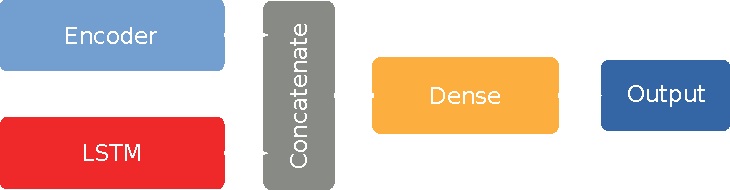
\includegraphics[width=0.9\textwidth]{figures/net_idea.pdf}
    \label{fig:network}
\end{figure}



\end{document}